% Chapter 2

\chapter{Data Analysis} % Main chapter title

\label{chapter:model} % For referencing the chapter elsewhere, use \ref{Chapter1} 
\lhead{Chapter 4. \emph{Model}} % This is for the header on each page - perhaps a shortened title
	
%----------------------------------------------------------------------------------------

Take the best genes ad simulate several times. Show bar plot of each gene, where the heights of the bars are the mean fitness, and with some brackets showing std of fitness.

\section{Dataset 1}

As a first step in the data analysis, it is useful to visualize the dataset. Figure 

The first attempt at PCA: The hope is that some regions in the parameter space correspond to regions in the fitness space. 
\begin{comment}
\begin{figure}
%issue 11
	\centering
	\subcaptionbox{\label{subfig:}}
	[0.49\linewidth]{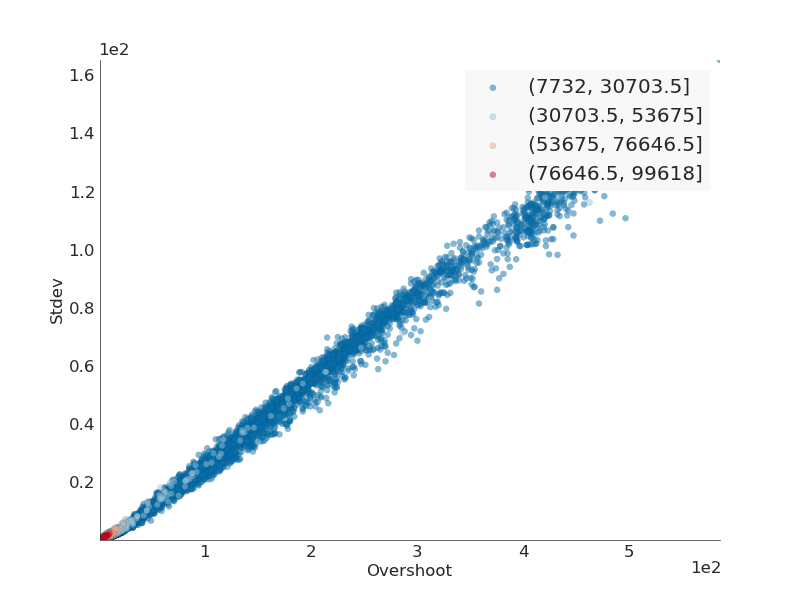
\includegraphics[width=0.6\textwidth]{issue_21_b.png}}
	\subcaptionbox{\label{subfig:}}
	[0.49\linewidth]{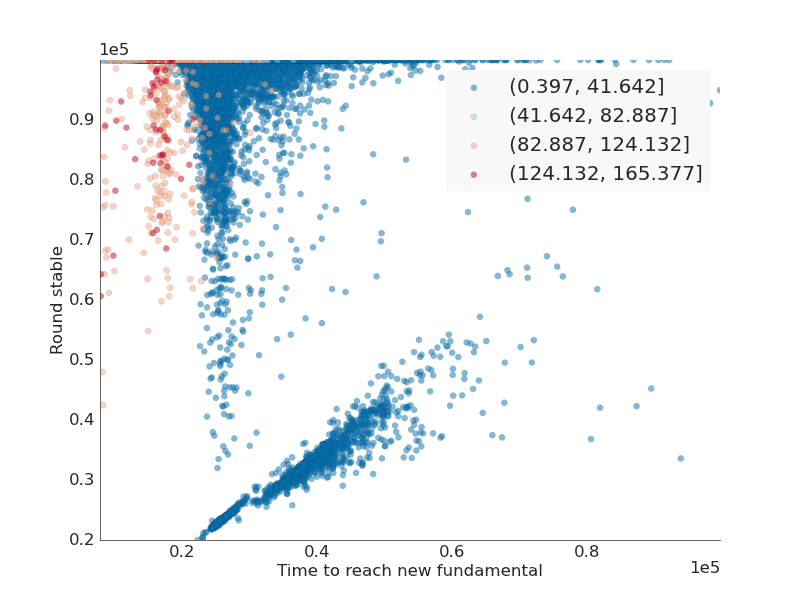
\includegraphics[width=0.6\textwidth]{issue_21_c.png}}
	\subcaptionbox{\label{subfig:}}
	[0.49\linewidth]{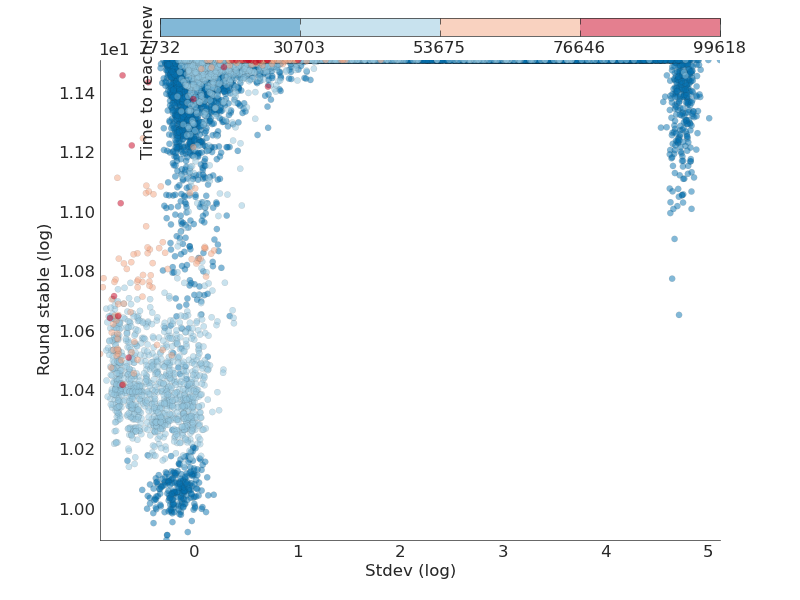
\includegraphics[width=0.6\textwidth]{issue_21_d.png}}
	\subcaptionbox{\label{subfig:}}
	[0.49\linewidth]{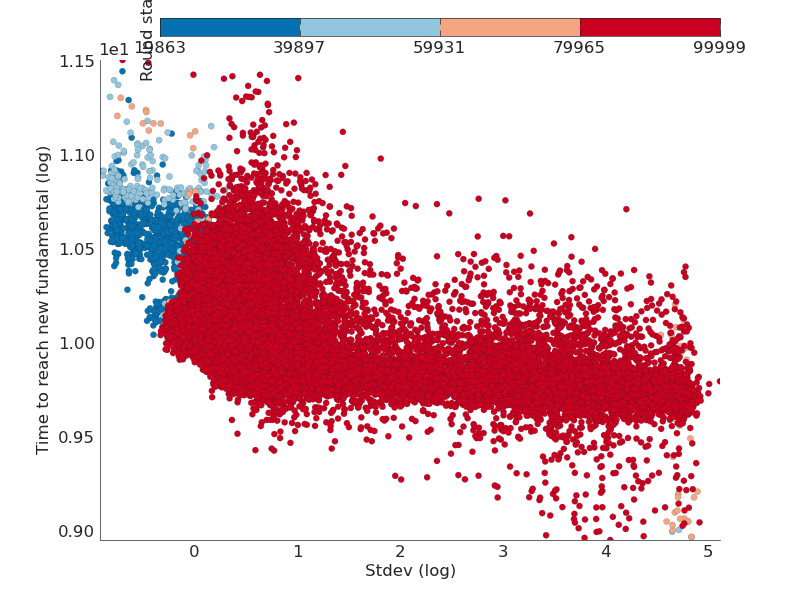
\includegraphics[width=0.6\textwidth]{issue_21_e.png}}

	\caption{Scatter plots for dataset 1}\label{fig:scatter_plot_dataset1}
	\label{sub:other_decompositions}
% subsection other_decompositions (end)
\end{figure}


\end{comment}
\begin{tabular}{lrrrr}
\toprule
{} &      c0 &      c1 &      c2 &      c3 \\
\midrule
sc\_latency\_mu                 &    41.9 &    55.3 &    40.8 &    54.5 \\
sc\_latency\_s                  &    27.5 &    30.0 &    22.7 &    29.7 \\
sc\_nAgents                    &    34.3 &    22.9 &    29.1 &    22.8 \\
sc\_think\_mu                   &   118.2 &   101.0 &   108.4 &   101.0 \\
sc\_think\_s                    &     9.0 &    14.8 &    20.8 &     7.5 \\
sc\_timehorizon\_mu             &  3372.8 &  2079.4 &  4352.3 &  1233.1 \\
sc\_timehorizon\_s              &  1394.6 &  1155.1 &  1365.0 &  1246.8 \\
sc\_waitTimeBetweenTrading\_mu  &     3.9 &     4.1 &     4.0 &     5.3 \\
sc\_waitTimeBetweenTrading\_s   &    11.8 &     9.0 &    12.8 &     8.6 \\
ssmm\_latency\_mu               &    10.1 &     7.8 &     9.3 &     8.0 \\
ssmm\_latency\_s                &     1.3 &     1.6 &     1.5 &     1.7 \\
ssmm\_nAgents                  &     6.3 &     3.0 &     4.4 &     2.5 \\
ssmm\_think\_mu                 &     6.7 &     6.2 &     6.6 &     6.2 \\
ssmm\_think\_s                  &     5.4 &     3.8 &     5.7 &     3.5 \\
overshoot                     &     3.4 &     3.1 &     3.3 &     3.2 \\
round\_stable                  & 44418.4 & 39518.4 & 40253.2 & 40769.0 \\
stdev                         &     0.9 &     0.8 &     0.9 &     0.9 \\
time\_to\_reach\_new\_fundamental & 29204.2 & 28132.4 & 28417.6 & 27735.5 \\
\bottomrule
\end{tabular}

\begin{table} \centering \begin{tabular}{lrrrr}
\toprule
{} &      c0 &      c1 &      c2 &      c3 \\
\midrule
\sclatencymu                &    27.9 &    17.1 &    25.3 &    26.2 \\
\sclatencys                 &    13.6 &     7.2 &    14.1 &    13.5 \\
\scnAgents                  &    71.2 &    29.2 &    47.7 &    52.8 \\
\scthinkmu                  &    29.6 &    21.7 &    28.6 &    24.6 \\
\scthinks                   &    16.9 &    17.9 &    18.7 &    19.1 \\
\sctimehorizonmu            &   465.0 &   461.3 &   428.1 &   343.2 \\
\sctimehorizons             &   602.7 &   240.9 &   236.7 &   672.6 \\
\scwaitTimeBetweenTradingmu &    13.8 &    10.9 &    11.8 &    14.7 \\
\scwaitTimeBetweenTradings  &     5.4 &     2.4 &     2.8 &     4.2 \\
\ssmmlatencymu              &     2.4 &     3.6 &     2.7 &     3.0 \\
\ssmmlatencys               &     1.6 &     2.3 &     1.8 &     2.0 \\
\ssmmnAgents                &     5.8 &     2.9 &     4.4 &     6.3 \\
\ssmmthinkmu                &     2.8 &     2.0 &     1.9 &     2.1 \\
\ssmmthinks                 &     1.5 &     1.5 &     1.6 &     1.5 \\
\overshoot                  &    10.3 &     5.3 &     7.9 &    11.5 \\
\roundstable                & 35978.1 & 23401.6 & 27605.3 & 30993.2 \\
\stdev                      &     2.3 &     1.2 &     1.9 &     3.1 \\
\timetoreachnewfundamental  &  6033.3 &  2642.4 &  4628.7 &  5330.8 \\
\bottomrule
\end{tabular}
 \label{issue_65_Std} \caption{s} \end{table}

\subsection{Other decompositions} % (fold)